\section{System Design and Methodology}

KBDebugger is a seven-stage pipeline for human-in-the-loop knowledge graph construction from regulatory documents. The system is grounded in three design principles: (i) \emph{graph-conditioned extraction} — every filtering and classification step is informed by the current graph state, not applied in isolation; (ii) \emph{deontic fidelity} — obligation strength is preserved as a first-class property of each triple, not normalized away; and (iii) \emph{append-only provenance} — the full source context of every triple is retained regardless of how many subsequent documents re-assert the same claim.

Figure~\ref{fig:architecture} provides an overview of the pipeline and its component stages.

\begin{figure}[t]
    \centering
    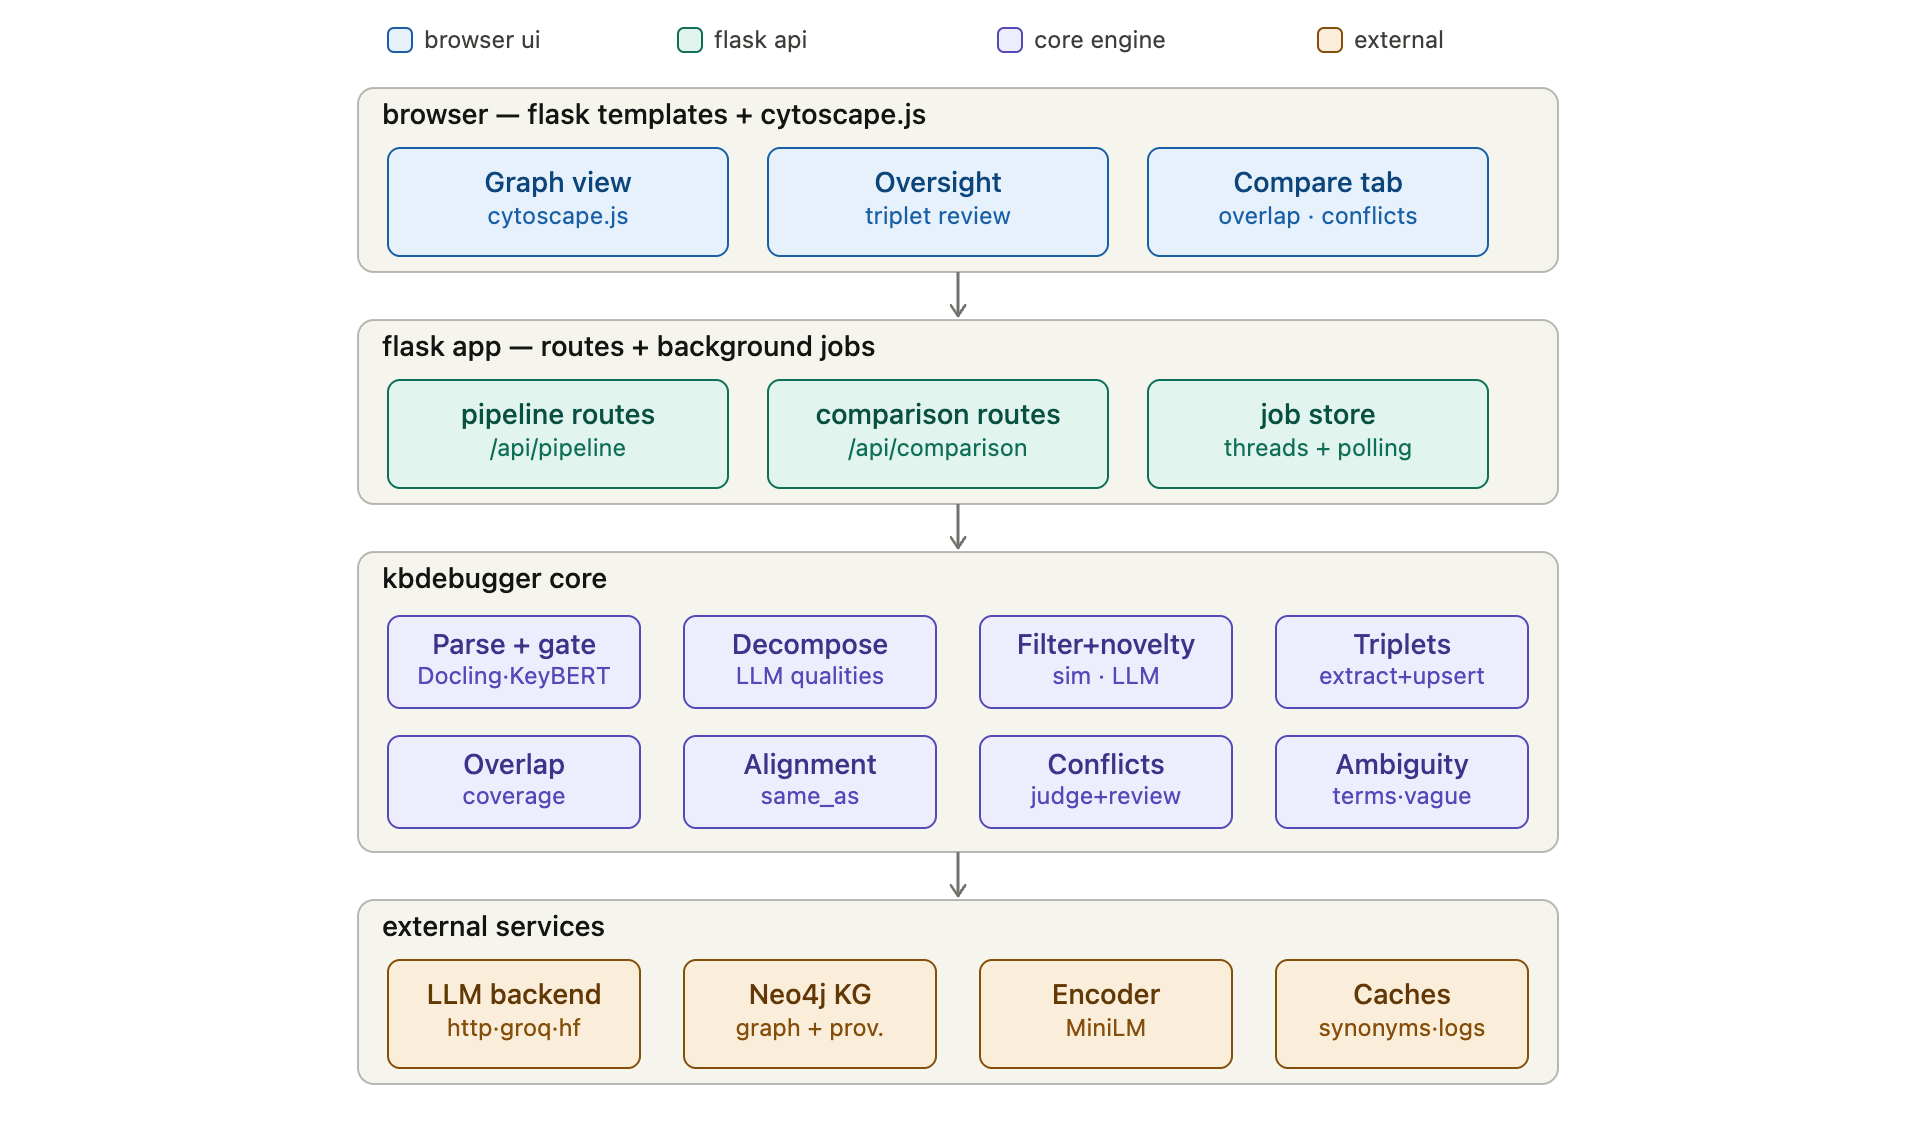
\includegraphics[width=\columnwidth]{Figures/method-overall-architecture.png}
    \caption{KBDebugger pipeline overview. Seven stages transform a regulatory PDF into provenance-tracked triples in a Neo4j knowledge graph, with human review at Stage 6 before any graph upsert.}
    \label{fig:architecture}
\end{figure}

\subsection{Stage 1: Graph-Context Retrieval}

Before any document is ingested, the system retrieves the relevant subgraph from the existing knowledge graph using keyword-guided pattern matching against node names, relation types, and stored provenance metadata in Neo4j. This subgraph serves as the semantic context against which new extractions are compared in Stages 3 and 4. The retrieval step ensures that extraction is not document-agnostic: the system knows what it already knows.

Retrieval is performed via three complementary patterns: keyword occurrence in source node name, in target node name, and in relationship type or sentence metadata. Results are deduplicated and limited to a configurable per-pattern count (default 50 relations per pattern) to prevent context bloat for densely interconnected topics.

\subsection{Stage 2: Document Ingestion and Quality Decomposition}

Stage 2 has three substages that transform a raw PDF into a set of \emph{atomic quality sentences} — the granular unit of analysis throughout the remainder of the pipeline.

\textbf{2a. Structure-Aware PDF Parsing.} The system uses Docling~\citep{docling2024} for layout-aware PDF parsing with optional OCR and table recognition. A conservative post-processing pass filters reference sections to prevent bibliographic noise from entering the extraction stream. Each paragraph is retained with its full provenance (page number, heading hierarchy, document title).

\textbf{2b. Keyword Filtering.} Paragraphs are filtered by relevance to the target dimension using KeyBERT~\citep{grootendorst2020keybert}, a sentence-transformer-based keyphrase extractor. The system supports three filtering modes: (i) a curated Trustworthy AI dimension keyword (e.g., \emph{fairness}, \emph{robustness}); (ii) user-supplied custom keywords with LLM-assisted synonym expansion and a persistent synonym cache; and (iii) whole-document extraction (no keyword gate). This stage substantially reduces the candidate set before the more expensive LLM stages.

\textbf{2c. Atomic Decomposition.} Each retained paragraph is decomposed into atomic quality sentences by an LLM. Conjunctions, lists, and compound obligations are split so that each output sentence encodes exactly one claim. This step is critical for downstream novelty classification: a compound sentence that mixes an existing claim with a novel qualifier would otherwise be classified as a single EXISTING unit. Decomposed sentences are batched (default 5 per LLM call) with optional parallelism for throughput.

Figure~\ref{fig:ingestion} illustrates the ingestion substages and the data shapes at each transition.

\begin{figure}[t]
    \centering
    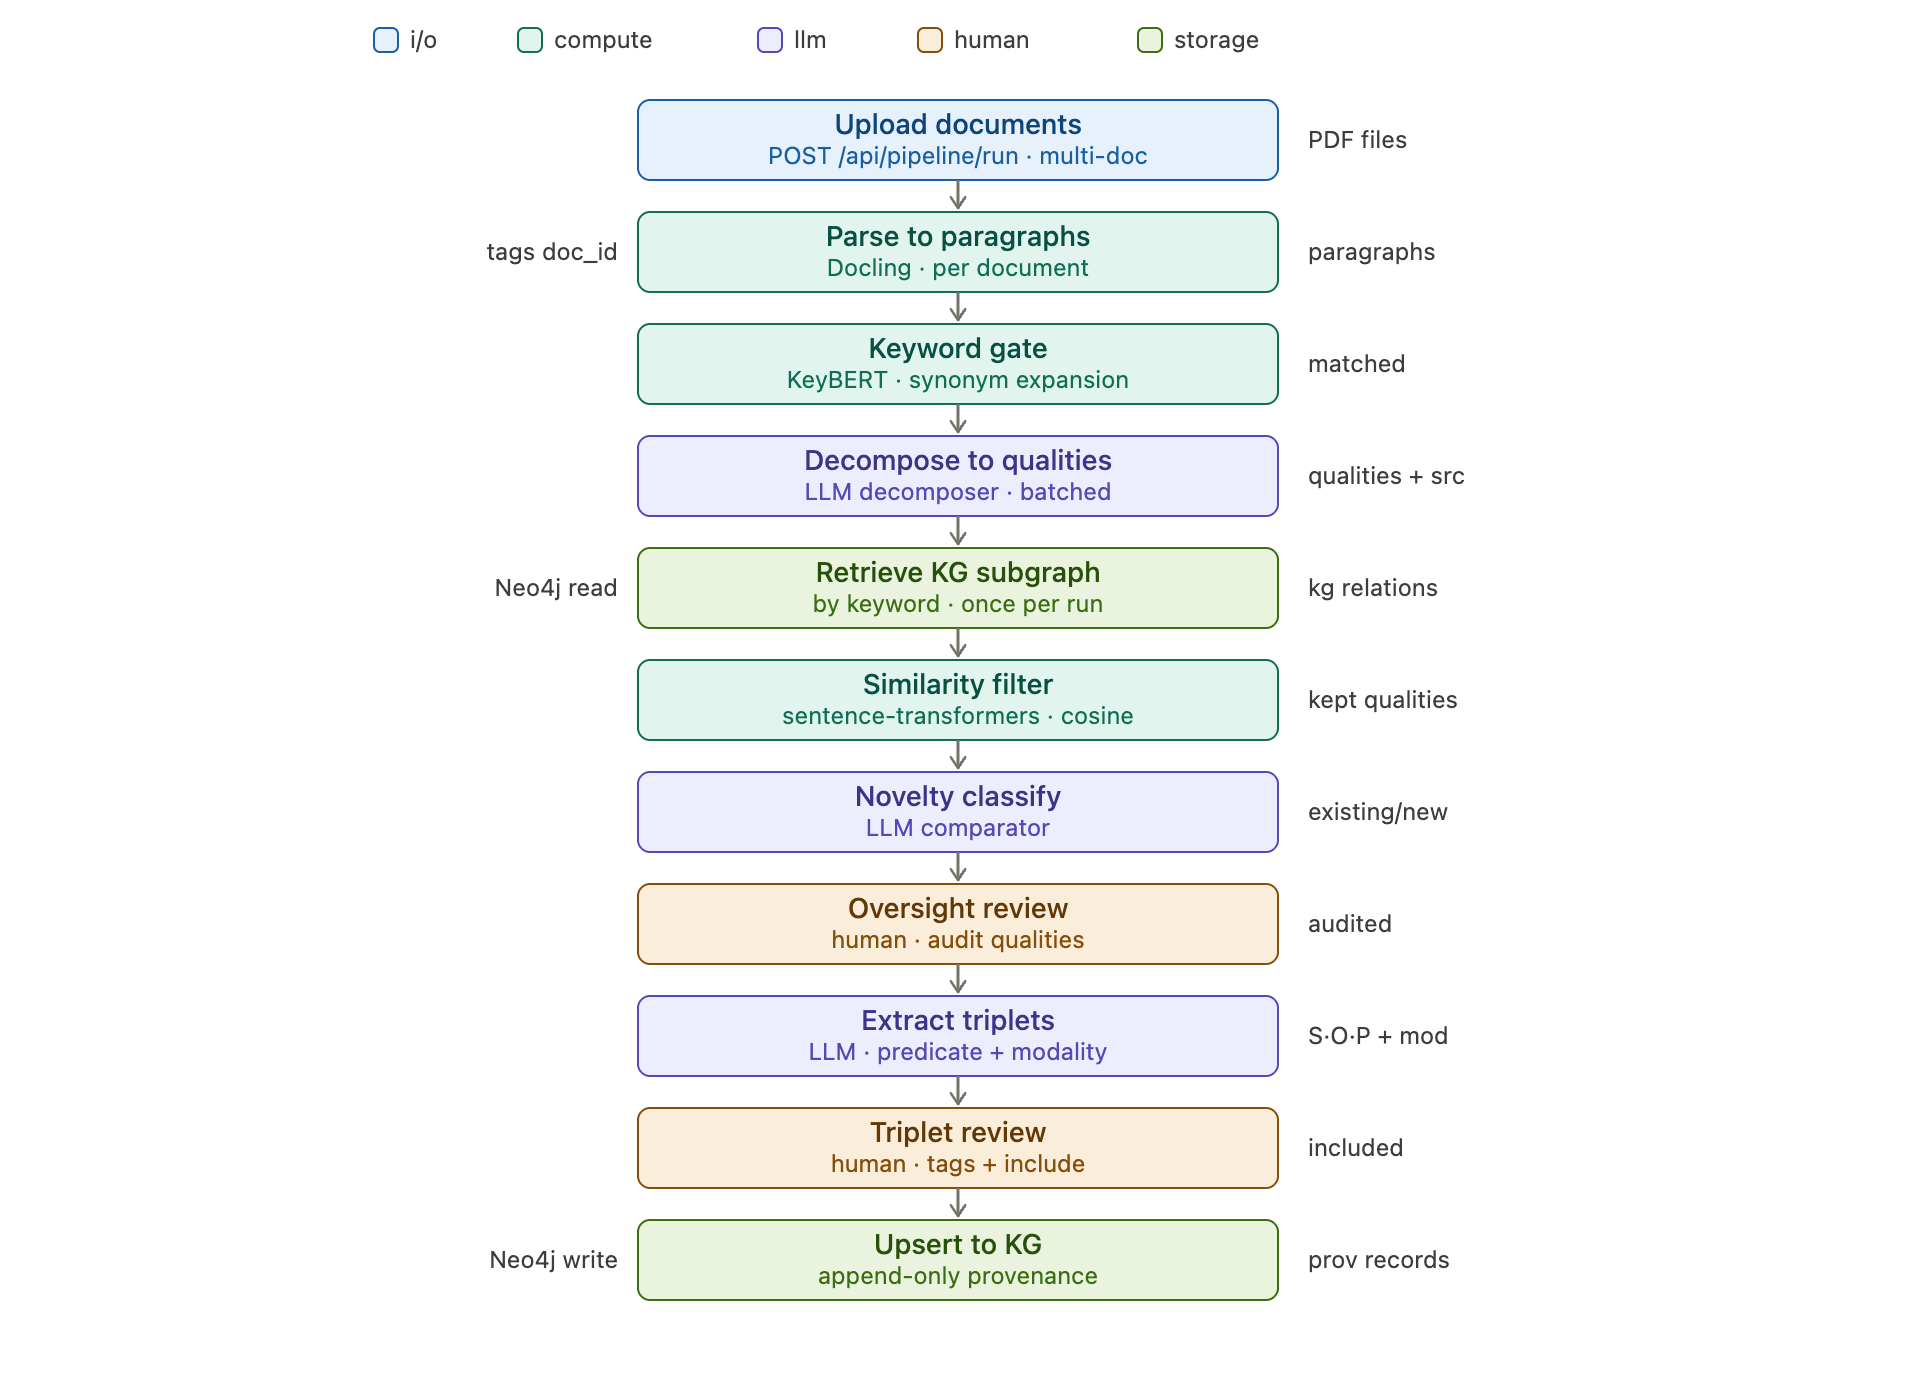
\includegraphics[width=\columnwidth]{Figures/method-ingestion-pipeline.png}
    \caption{Stage 2 ingestion substages: PDF parsing (Docling), keyword-gate filtering (KeyBERT), and atomic quality decomposition (LLM). Each substage reduces the candidate set and increases semantic granularity.}
    \label{fig:ingestion}
\end{figure}

\subsection{Stage 3: Node-Entity Similarity Filter}

Stage 3 filters atomic quality sentences by semantic proximity to the retrieved subgraph, retaining only those whose content overlaps meaningfully with concepts already represented in the KG. The system implements two filtering modes:

\textbf{Sentence mode} embeds each quality sentence and each KG relation sentence with a SentenceTransformer model~\citep{reimers2019sentencebert} (\texttt{all-MiniLM-L6-v2}) and retains qualities whose cosine similarity to at least one KG neighbor exceeds a configurable threshold (default 0.55).

\textbf{Node-entity mode} (default) extracts keyphrases from each quality sentence via KeyBERT (max 3-gram, top 8 per sentence), then computes cosine similarity between these entity embeddings and KG node name embeddings. This is more efficient than full-sentence comparison and better suited to ontology-style KGs where node names are short labels rather than full sentences. Qualities whose extracted entities match at least one KG node above threshold are retained; the matched nodes become the \emph{nearest neighbors} passed to Stage 4.

Figure~\ref{fig:nodefilter} illustrates the node-entity matching mechanism.

\begin{figure}[t]
    \centering
    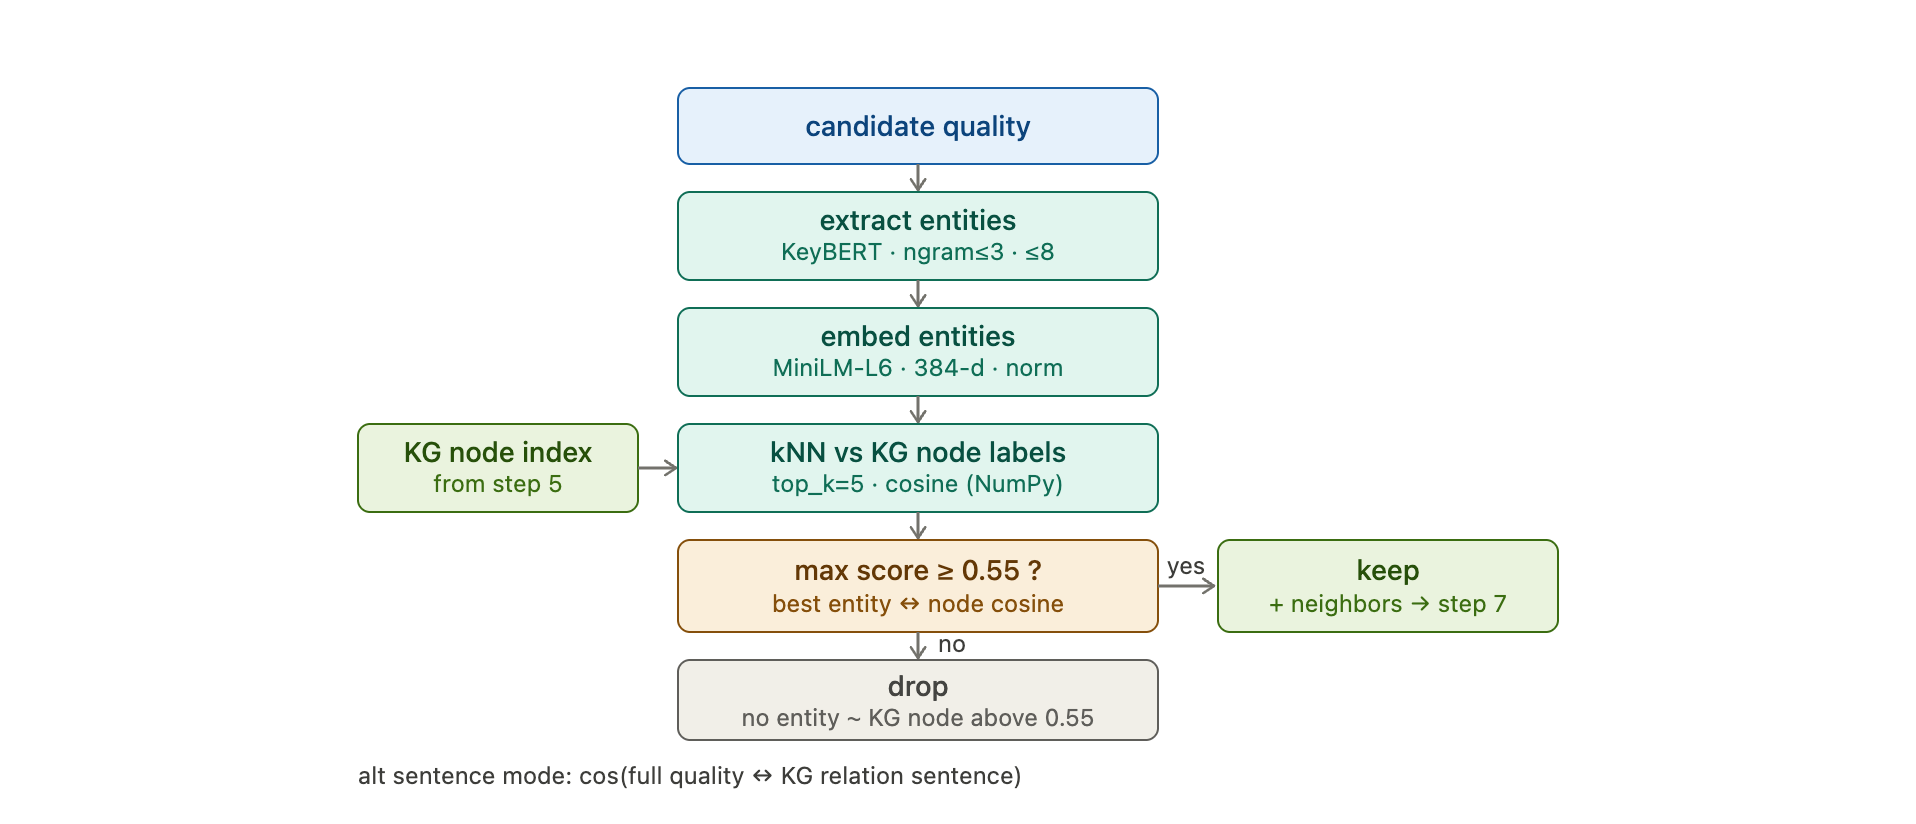
\includegraphics[width=\columnwidth]{Figures/method-node-entity-filter.png}
    \caption{Node-entity similarity filter. Keyphrases extracted from each quality sentence are embedded and matched against KG node name embeddings. Only qualities with at least one neighbor above the similarity threshold proceed to novelty classification.}
    \label{fig:nodefilter}
\end{figure}

\subsection{Stage 4: LLM Novelty Classification}

Each quality sentence that passes Stage 3 is classified by an LLM as one of three novelty categories:

\begin{itemize}
    \item \textbf{EXISTING}: The quality's semantic content is already fully captured by its nearest KG neighbors. No meaningful new information.
    \item \textbf{PARTIALLY\_NEW}: The quality overlaps with neighbors but adds a meaningful qualifier, scope restriction, condition, or new concept not currently in the graph.
    \item \textbf{NEW}: The quality introduces claims or relations not substantively covered by the retrieved subgraph.
\end{itemize}

The LLM prompt includes the quality sentence, the top-$k$ nearest KG neighbors (as full relation sentences with source metadata), and four few-shot examples spanning all three categories. The model is prompted at temperature 0.0 for deterministic classification and must return a structured JSON response including: the decision, a rationale, the novel spans (for PARTIALLY\_NEW/NEW), the most similar neighbor, and a confidence score (0--1). Novelty classification is the primary mechanism by which KBDebugger avoids re-extracting content already in the graph.

Figure~\ref{fig:novelty} shows the decision logic and output schema for this stage.

\begin{figure}[t]
    \centering
    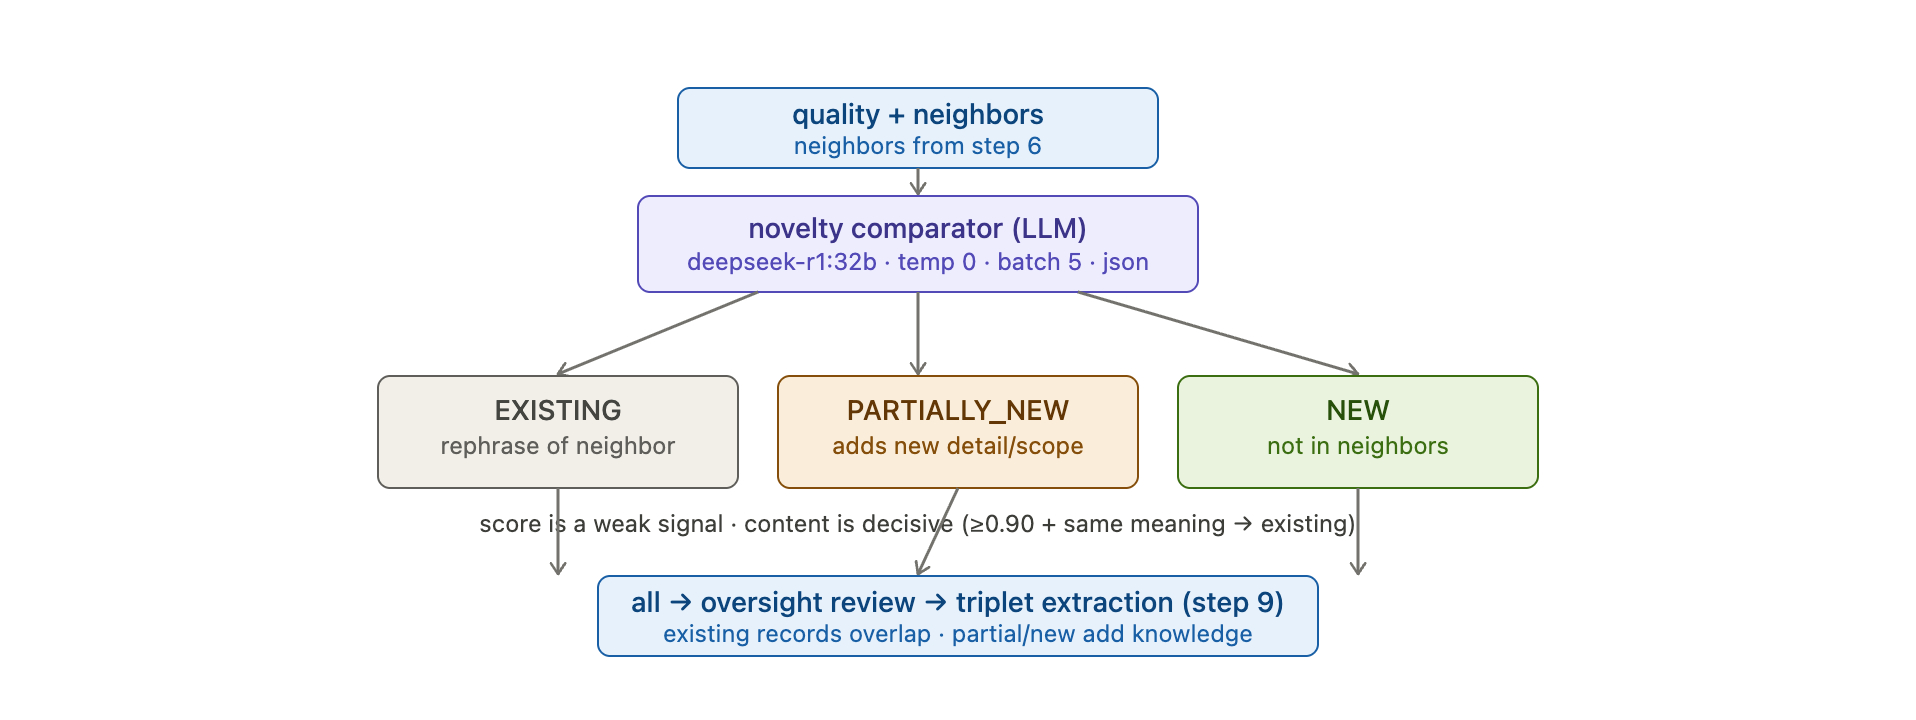
\includegraphics[width=\columnwidth]{Figures/method-novelty-decision.png}
    \caption{Novelty classification decision logic. The LLM receives the quality sentence, its nearest KG neighbors, and few-shot examples, then classifies the quality as EXISTING, PARTIALLY\_NEW, or NEW with supporting rationale.}
    \label{fig:novelty}
\end{figure}

\subsection{Stage 5: Controlled-Vocabulary Triplet Extraction}

Qualities classified as PARTIALLY\_NEW or NEW are forwarded to controlled-vocabulary triplet extraction. Unlike free-form OpenIE or KGGen-style extraction, KBDebugger constrains the predicate to one of four ontology families:

\begin{itemize}
    \item \textbf{Normative} (standards language): \texttt{Requires}, \texttt{Recommends}, \texttt{Permits}, \texttt{Prohibits}, \texttt{Defines}, \texttt{Provides}, \texttt{AppliesTo}, \texttt{Constrains}, \texttt{Measures}
    \item \textbf{Trustworthy AI dimensions}: \texttt{IsDimensionOf}, \texttt{ContributesTo}, \texttt{MightMitigate}, \texttt{MightIntroduce}, \texttt{SurfacesRisk}, \texttt{IsThreatTo}
    \item \textbf{Data science}: \texttt{Implements}, \texttt{HasParameter}, \texttt{HasInput}, \texttt{HasOutput}, \texttt{Evaluates}, \texttt{Performs}
    \item \textbf{Taxonomy}: \texttt{IsSubclassOf}, \texttt{IsEquivalentTo}, \texttt{IsA}
\end{itemize}

Triplet extraction also identifies \emph{deontic modality} from the wording of each quality sentence: \texttt{MANDATORY} (shall/must), \texttt{RECOMMENDED} (should), \texttt{OPTIONAL} (may/can), \texttt{PROHIBITED} (shall not/must not), or \texttt{NONE} for descriptive statements. Modality is recorded as a property on each extracted triple.

An optional schema grounding step passes a summary of the current Neo4j schema (existing node types, relation types, and templates) to the extraction prompt, biasing the LLM toward predicates and node labels already in use. Triplets whose content cannot be mapped to any allowed predicate are tagged \texttt{No schema fit} and excluded unless the reviewer overrides; off-vocabulary predicates are tagged \texttt{Needs schema review}.

\subsection{Stage 6: Pre-Merge KB Preview and Human Review}

Before any graph write, each proposed triplet is classified against the live knowledge graph
via a read-only \emph{pre-merge preview}. The preview assigns each triple one of five
categories:

\begin{itemize}
    \item \textbf{NEW} — the $(S, P, O)$ combination is not yet in the graph (concepts may
    already exist as nodes but the relation is new).
    \item \textbf{EXISTING} — an identical or equivalent triple is already present, with the
    same predicate and compatible modality.
    \item \textbf{TENSION} — the same $(S, P, O)$ exists but with a different deontic
    obligation strength (e.g.\ this document says MANDATORY, the graph says RECOMMENDED).
    \item \textbf{CONFLICT} — the same subject-object pair is already linked by a directly
    contradicting predicate (e.g.\ \texttt{Requires} vs.\ \texttt{Prohibits}).
    \item \textbf{RELATED} — the same concept pair is related in the graph but via a
    different, non-contradicting predicate.
\end{itemize}

The preview surfaces the KB-side sentence alongside the candidate triple so the reviewer can
compare the actual textual evidence, not just node names. CONFLICT and TENSION items are
sorted to the top of the review queue, directing reviewer attention to the decisions with
the highest consequence. This pre-merge gate is the primary mechanism by which
KBDebugger detects cross-document obligation conflicts at the point of insertion —
before they are committed to the graph.

All proposed triplets, with their preview categories, are then presented to a human reviewer.
The review interface shows: the source document, chunk index, original quality sentence,
nearest KG match from Stage~3, similarity score, the proposed $(S, P, O)$ triple,
deontic modality, novelty class, schema status, and the pre-merge category. Reviewers
can include, edit, or reject each triplet; edits can correct predicate choice, entity
label, or modality before submission. Reviewer decisions are exported in an auditable
XLSX workbook.

\subsection{Stage 7: Knowledge Graph Upsert}

Accepted triplets are upserted into Neo4j using \texttt{MERGE} semantics on the $(S, P, O)$
key. The system implements append-only provenance: each upsert appends a provenance record
(document name, quality sentence, chunk index, source excerpt, modality) to the edge. Triples
asserted by multiple documents accumulate evidence across all source documents without
duplication. Nodes are created as labeled entities (\texttt{:Node\{name\}}) and relations as
native Neo4j relationship types.

\subsection{Stage 8: Five-Strategy Graph Verification}

After each upsert, a read-only verifier checks the graph against five quality strategies:

\begin{itemize}
    \item \textbf{S1 Coverage ($\tau \geq 0.90$)} — at least 90\% of source sentences are
    reflected in $\geq 1$ triple (verified via provenance record matching).
    \item \textbf{S2 Correctness ($\tau = 1.0$)} — all nodes have non-placeholder names and
    all edges use a predicate from the declared vocabulary.
    \item \textbf{S3 Consistency ($\tau = 1.0$)} — no $(S, O)$ pair is simultaneously linked
    by both an affirmative predicate (Requires, Recommends, Permits) and a prohibitive one
    (Prohibits).
    \item \textbf{S4 Completeness ($\tau = 1.0$)} — every triple has non-empty subject, object,
    and predicate, and at least one provenance record.
    \item \textbf{S5 Minimality ($\tau = 1.0$)} — no duplicate $(S, P, O)$ edge exists in
    the graph.
\end{itemize}

Each strategy is isolated in its own exception handler; a single failing check degrades to a
per-strategy error rather than aborting the entire verdict. The verifier emits a global
PASS/FAIL verdict alongside per-strategy scores, summaries, and flagged triples — providing
a complete, reproducible audit trail for each ingestion session. This post-upsert verification
step closes the quality loop: extraction errors that pass human review (e.g.\ a reviewer
accepting a duplicate by mistake) are still caught before the graph is used for downstream
compliance reasoning.

\subsection{Multi-Document Comparison Engine}

After two or more documents have been ingested, the comparison engine supports four analyses across the unified KG:

\textbf{Overlap \& Coverage} computes per-document assertion counts, concept breadth, and a concept-by-document matrix showing which concepts are addressed by which standards and how many triples each standard contributes to shared concepts.

\textbf{Semantic Alignment} proposes \texttt{SAME\_AS} equivalences between nodes from different documents whose embeddings exceed a configurable cosine threshold (default 0.78). Reviewers accept (creating a \texttt{:same\_as} edge for canonicalization) or reject (creating a \texttt{:not\_same\_as} edge, preventing the pair from resurfacing).

\textbf{Conflict Detection} surfaces four conflict types: (i) \emph{obligation conflict} — same $(S, P, O)$ with different modality across documents; (ii) \emph{definition divergence} — same concept defined differently; (iii) \emph{taxonomy conflict} — reversals in subsumption hierarchy; (iv) \emph{value conflict} — same subject and predicate, different object values. Each candidate is judged by an LLM (AGREE / UNRELATED / TENSION / CONTRADICT + rationale), and confirmed conflicts are written as \texttt{:Conflict} nodes in the graph.

\textbf{Normative Gap Detection} identifies concepts that appear in MANDATORY or RECOMMENDED assertions but are never given a formal definition (\texttt{Defines} predicate) within the same document. These \emph{normatively obligated but undefined} concepts represent the gap between what a standard requires and what it explains, directly answering RQ1.

Figure~\ref{fig:comparison} shows the comparison engine UI and its four analysis tabs.

\begin{figure}[t]
    \centering
    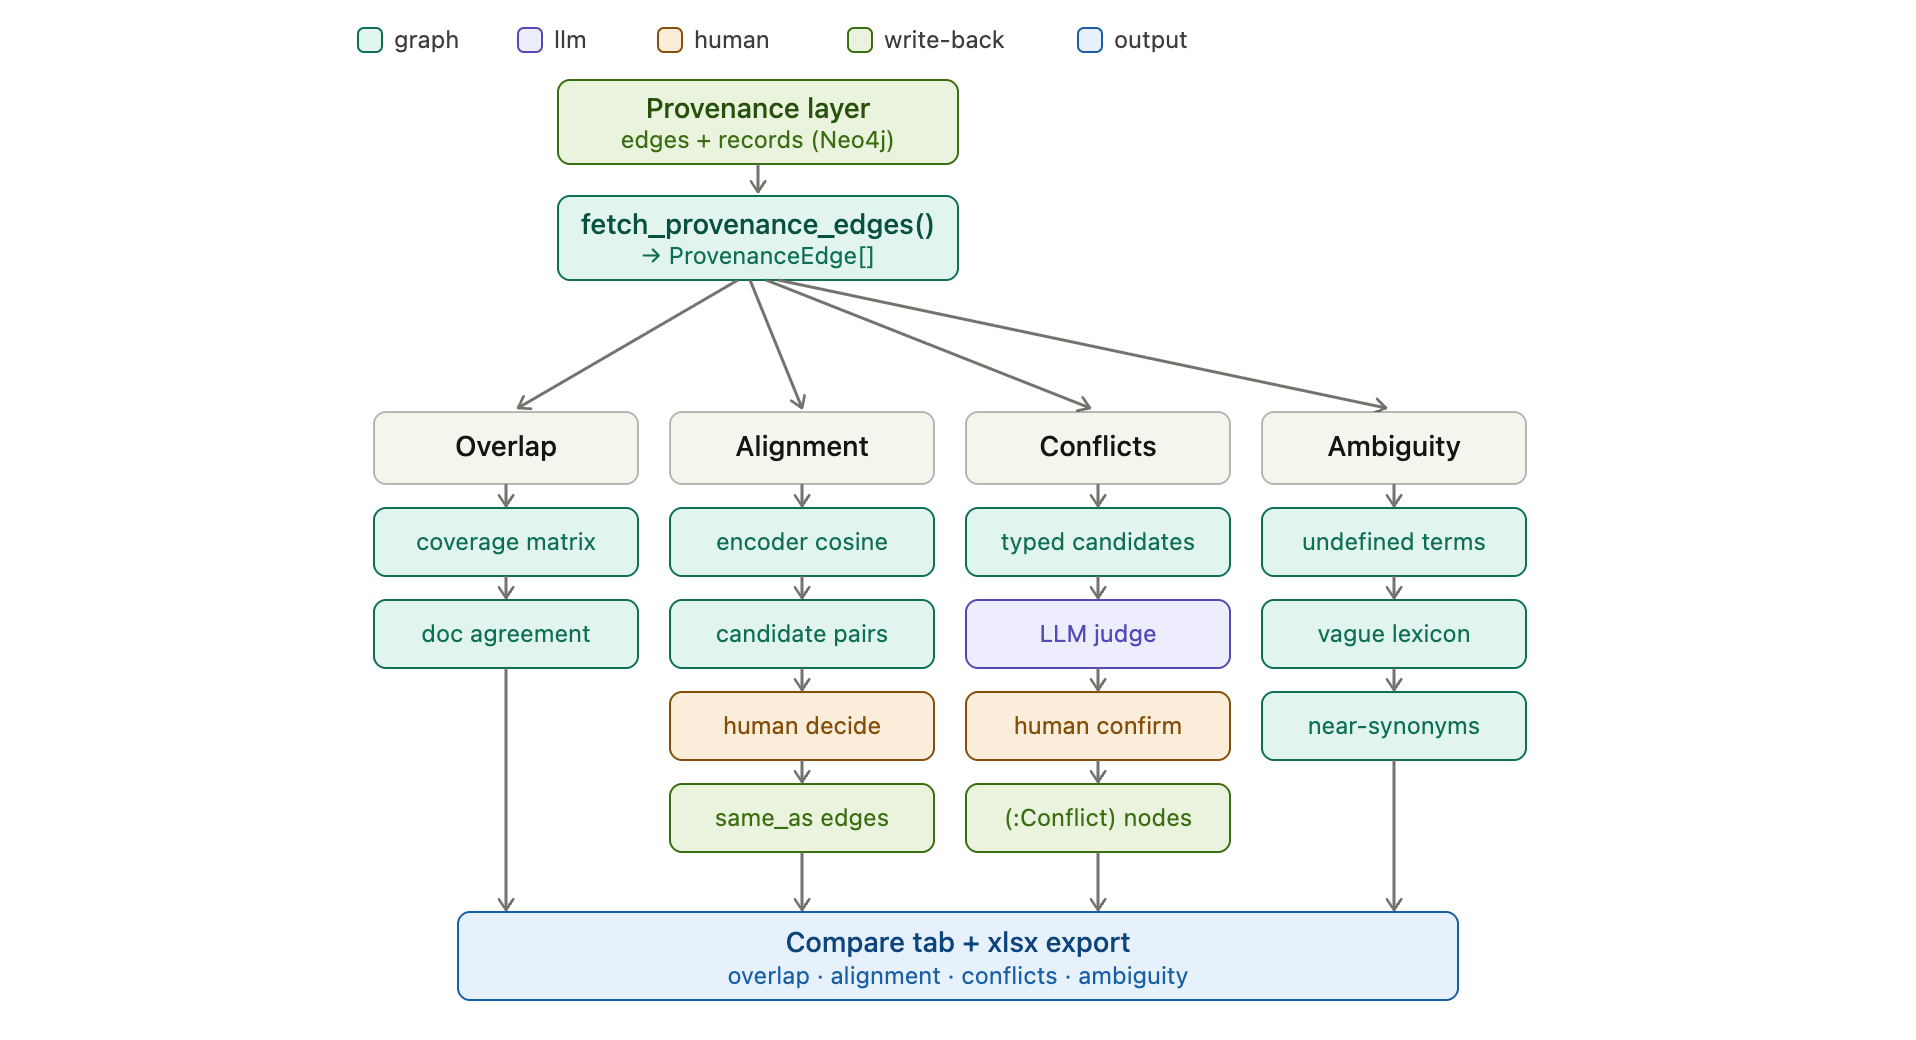
\includegraphics[width=\columnwidth]{Figures/method-comparison-engine.png}
    \caption{Comparison engine: four analysis views (Overlap, Alignment, Conflicts, Ambiguity) applied to a KG built from multiple standards. The Conflicts tab flags obligation conflicts across documents; the Ambiguity tab flags normative gaps.}
    \label{fig:comparison}
\end{figure}
